\chapter{Planification}

\section{Methodology}
Usually in the degree, we use a waterfall model to develop. For small projects and use cases this methodology \\
works fine, but in bigger projects it carries a lot of issues. \\

In addition, it does not make sense to design all the system in earlier iterations, due to the fact that I \\
don't really have much experience using these technologies, so my diagrams will change a lot in the future. \\
This way, I should mantein both codebase and designs, and designs will be changed a lot and won't be very useful. \\

In conclusion, although waterfall model is the most used in the degree, I opted to use an agile methodology and reiterate \\
the design process, so I'm flexible and I only design what it is really neccessary to me in order to develop the app and mantein the codebase later on. \\

At first, I used a process similar to waterfall model. I captured all the requirements, I design in a very basic way the app and I started developing the architecture. \\
Later on, I would change the design, and the architecture itself, but that will come in the implementation chapter later. \\

\begin{figure}[H]
    \begin{center}
        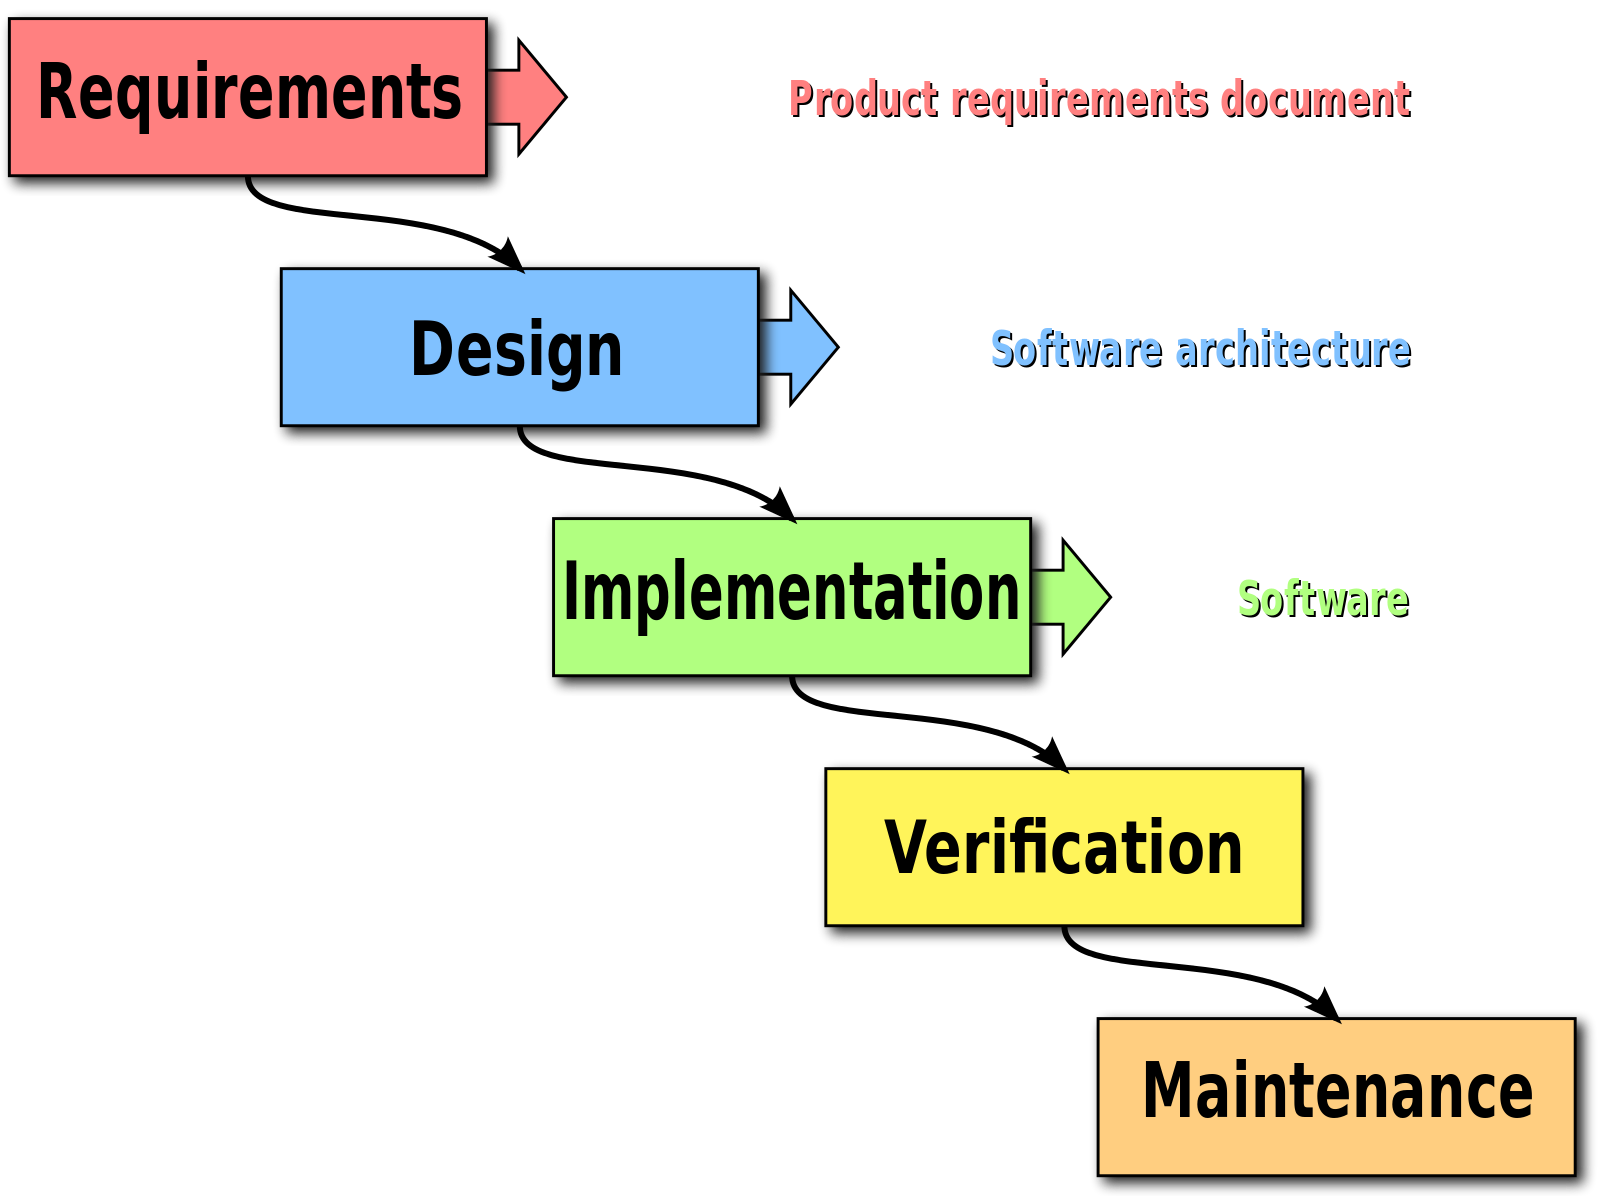
\includegraphics[width=0.4\textwidth]{assets/waterfall_model.png}
        \caption{Waterfall Model. \cite{Waterfall}}
        \label{fig:planification_waterfall_model}
    \end{center}
\end{figure}

In the Scrum model we iterate every fixed amount of time and start a new waterfall model. \\
We critize what could be changed to implement and develop in a better way and we reorder the tasks. \\
Me, instead of having fixed sprints, I used this methodology but the amount of time of every sprint was flexible. It was the neccessary time in order to achieve a new product with a value increase. \\

\begin{figure}[H]
    \begin{center}
        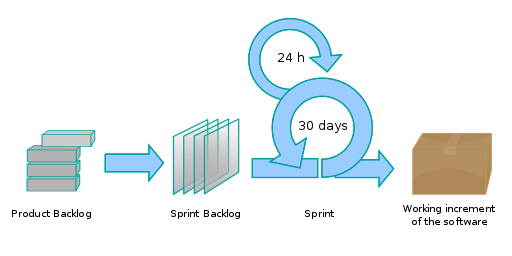
\includegraphics[width=0.4\textwidth]{assets/scrum.png}
        \caption{Scrum Model. \cite{Scrum}}
        \label{fig:planification_scrum_model}
    \end{center}
\end{figure}

Firstly, I recognised all the tasks that I should complete in order to develop the application and the thesis itself. I divided into groups:
\begin{itemize}
    \item Literature review
    \item Backend
    \item Frontend
    \item Deep Learning service
    \item Documentation
    \item Design
\end{itemize}

Then I grouped the tasks in order to deliver a new product that represents a value increase. \\
This new product should be validated, so a meeting with the tutor was appointed. \\
Then, the rest of the active tasks were given a priority and grouped to form the new iteration backlog. \\
There were a lot of replanification, this was due to:
\begin{itemize}
    \item Unexperience. I was not able to correctly planificate the tasks, although I splitted them into smaller ones. I was sometimes stuck in some of them and others required less work load than expected.
    \item Flexible temporization. I was aware of my lack of experience and that I was going to fail in this task, so I tried to bring my deadline earlier so that I had more time.
    \item Subjects: In my Erasmus University we had some subjects in which we studied in depth C-Sharp, ASP.NET core and React Native. I was not aware of it, so I replanificated my tasks related to this thesis so that I could work on them after studying the technology in the subject to gain time.
    \item Uncertainties: Travels, plans, exams, deadline from the university, technical interviews...
\end{itemize}

\section{Temporarization}
In order to create my temporization, I used Notion \cite{Notion}. You can check my planifications \href{https://cyclic-chiller-238.notion.site/LearnASL-60bb8f91ed8f4ccfa90f98ee2306403d}{here}. \\

\subsection{Theorical temporization}
\begin{table}[H]
    \centering
    \resizebox{\textwidth}{!}{
    \begin{tabular}{|l|l|l|l|}
        \cline{1-4}      Name                                &    Milestone                                                              &    Due                                           &       State   \\
        \hline           Project set up                      &    \href{https://github.com/JesusGonzalezA/LearnASL/milestone/1}{Link}      &    November 12, 2021                             &       No      \\
        \hline           Graphical Stats                     &    \href{https://github.com/JesusGonzalezA/LearnASL/milestone/8}{Link}      &    February 4, 2022    →   February 11, 2022     &       No      \\
        \hline           The app saves info                  &    \href{https://github.com/JesusGonzalezA/LearnASL/milestone/7}{Link}      &    January 7, 2022     →   January 14, 2022      &       No      \\
        \hline           The app can create tests            &    \href{https://github.com/JesusGonzalezA/LearnASL/milestone/4}{Link}      &    December 31, 2021   →   January 7, 2022       &       No      \\
        \hline           Frontend avalaible                  &    \href{https://github.com/JesusGonzalezA/LearnASL/milestone/3}{Link}      &    December 10, 2021   →   December 31, 2021     &       No      \\
        \hline           The app is designed                 &    \href{https://github.com/JesusGonzalezA/LearnASL/milestone/2}{Link}      &    December 3, 2021    →   December 17, 2021     &       No      \\
        \hline           The user is authenticated           &    \href{https://github.com/JesusGonzalezA/LearnASL/milestone/6}{Link}      &    November 12, 2021   →   December 3, 2021      &       No      \\
        \hline           The app validates the videos        &    \href{https://github.com/JesusGonzalezA/LearnASL/milestone/5}{Link}      &    February 11, 2022   →   February 25, 2022     &       No      \\
        \hline           Using own ML model                  &    \href{https://github.com/JesusGonzalezA/LearnASL/milestone/10}{Link}     &                                                  &       No      \\
        \hline           Migrating to React Native or PWA    &    \href{https://github.com/JesusGonzalezA/LearnASL/milestone/9}{Link}      &                                                  &       No      \\
        \hline
    \end{tabular}
    }
\caption{Theorical temporization}
\label{table:planification_theorical_temporization}
\end{table}

\subsection{Real temporization}
I changed the order of the milestones. I decided to develop the backend of the application first, instead of the frontend or implementing them in the same time. \\

This decision was made because focusing on the same technology would allow me to go faster because I don't have to change the context and I was learning ASP.NET core in my  \\
university, so I could ask my teachers for help and it also helped me to study. \\
\begin{table}[H]
    \centering
    \resizebox{\textwidth}{!}{
    \begin{tabular}{|l|l|l|l|l|}
        \cline{1-5}      Name                                           &    Milestone                                              &       Due                                     & State & Tag       \\
        \hline           Project set up                                 & \href{https://github.com/JesusGonzalezA/LearnASL/milestone/1}{Link}    &       November 12, 2021                       & Yes   & Backend, Frontend \\
        \hline           Implement authorization and authentication     & \href{https://github.com/JesusGonzalezA/LearnASL/milestone/6}{Link}    &       November 12, 2021 → December 3, 2021    & Yes   & Backend   \\
        \hline           The app can create tests: just word to video   &                                                        &       December 3, 2021  → January 7, 2022      & No    & Backend   \\
        \hline           The app can create the rest of tests           & \href{https://github.com/JesusGonzalezA/LearnASL/milestone/4}{Link}    &       January 7, 2022   → January 21, 2022      & No    & Backend   \\
        \hline           The app create stats                           & \href{https://github.com/JesusGonzalezA/LearnASL/milestone/8}{Link}    &       January 21, 2022  → January 28, 2022     & No    & Backend   \\
        \hline           The app is designed                            & \href{https://github.com/JesusGonzalezA/LearnASL/milestone/2}{Link}    &       January 28, 2022  → February 4, 2022     & No    & Frontend  \\
        \hline           Frontend avalaible                             & \href{https://github.com/JesusGonzalezA/LearnASL/milestone/3}{Link}    &       February 4, 2022  → March 4, 2022        & No    & Frontend  \\
        \hline           Connect frontend and backend                   &                                                         &       March 4, 2022     → March 11, 2022          & No    & Frontend  \\
        \hline           The app validates the videos                   & \href{https://github.com/JesusGonzalezA/LearnASL/milestone/5}{Link}    &       March 11, 2022    → April 1, 2022          & No    & Backend   \\
        \hline           Using own ML model                             & \href{https://github.com/JesusGonzalezA/LearnASL/milestone/10}{Link}   &                                               & No    & Backend   \\
        \hline           Migrating to React Native or PWA               & \href{https://github.com/JesusGonzalezA/LearnASL/milestone/9}{Link}    &                                               & No    & Frontend  \\
        \hline
    \end{tabular}
    }
\caption{Modification v1}
\label{table:planification_real_v1}
\end{table}

The next modification was made because I did not take into account the task of documenting what I was implementing, and I had to divide the task in \textit{Frontend} as well. \\

Also, I underestimated how much time doing unit tests was going to take me. This was because in the subject we were going to learn them in depth, but we finally did not \\
focused on one single framework, so I had to learnt it by myself. \\
\begin{table}[H]
    \centering
    \resizebox{\textwidth}{!}{
    \begin{tabular}{|l|l|l|l|l|}
        \cline{1-5}      Name                                           &    Milestone                                              &       Due   & State & Tag  \\
        \hline Project set up & \href{https://github.com/JesusGonzalezA/LearnASL/milestone/1}{Link} & November 12, 2021 & Yes & Backend, Frontend    \\
        \hline Implement authorization and authentication & \href{https://github.com/JesusGonzalezA/LearnASL/milestone/6}{Link} & November 12, 2021 → December 3, 2021 & Yes & Backend   \\
        \hline The app can create tests & \href{https://github.com/JesusGonzalezA/LearnASL/milestone/4}{Link} & December 3, 2021 → January 7, 2022 & Yes & Backend   \\
        \hline The app create stats & \href{https://github.com/JesusGonzalezA/LearnASL/milestone/8}{Link} & January 1, 202 → January 7, 202 & Yes & Backend  \\
        \hline Documentate &  & January 6, 2022 → January 11, 2022 & Yes & Backend  \\
        \hline Integration tests api &  & January 12, 2022 → January 26, 2022 & No & Backend    \\
        \hline The app is designed & \href{https://github.com/JesusGonzalezA/LearnASL/milestone/2}{Link} & January 26, 2022 → February 4, 2022 & No & Frontend   \\
        \hline User management &  & February 4, 2022 → February 11, 2022 & No & Frontend    \\
        \hline Test management &  & February 11, 2022 → February 21, 2022 & No & Frontend   \\
        \hline Stats management &  & February 21, 2022 → February 28, 2022 & No & Frontend  \\
        \hline The app validates the videos & \href{https://github.com/JesusGonzalezA/LearnASL/milestone/5}{Link} & February 28, 2022 → March 20, 2022 & No & Backend    \\
        \hline Using own ML model & \href{https://github.com/JesusGonzalezA/LearnASL/milestone/10}{Link} &  & No & Backend   \\
        \hline Migrating to React Native or PWA & \href{https://github.com/JesusGonzalezA/LearnASL/milestone/9}{Link} &  & No & Frontend \\
        \hline Integrate with google analytics &  &  & No & Frontend \\
        \hline
    \end{tabular}
    }
\caption{Modification v2}
\label{table:planification_real_v2}
\end{table}

This modification was made due to a good new. Doing the unit tests, after learning the framework, did not take me that amount of time. \\

Therefore, I modify the planification to rest some days and dedicate myself to design the app more days. \\
\begin{table}[H]
    \centering
    \resizebox{\textwidth}{!}{
    \begin{tabular}{|l|l|l|l|l|}
        \cline{1-5}      Name                                           &    Milestone                                              &       Due   & State & Tag  \\
        \hline Project set up & \href{https://github.com/JesusGonzalezA/LearnASL/milestone/1}{Link} & November 12 , 2021 & Yes & Backend, Frontend \\
        \hline Implement authorization and authentication & \href{https://github.com/JesusGonzalezA/LearnASL/milestone/6}{Link} & November 12 , 2021 → December 3 , 2021 & Yes & Backend \\
        \hline The app can create tests & \href{https://github.com/JesusGonzalezA/LearnASL/milestone/4}{Link} & December 3 , 2021 → January 7 , 2022 & Yes & Backend \\
        \hline The app create stats & \href{https://github.com/JesusGonzalezA/LearnASL/milestone/8}{Link} & January 1 , 202 → January 7 , 202 & Yes & Backend \\
        \hline Documentate &  & January 6 , 2022 → January 11 , 2022 & Yes & Backend \\
        \hline Integration tests api &  & January 12 , 2022 → January 15 , 2022 & Yes & Backend \\
        \hline The app is designed & \href{https://github.com/JesusGonzalezA/LearnASL/milestone/2}{Link} & January 18 , 2022 → February 4 , 2022 & No & Frontend \\
        \hline User management &  & February 4 , 2022 → February 11 , 2022 & No & Frontend \\
        \hline Test management &  & February 11 , 2022 → February 21 , 2022 & No & Frontend \\
        \hline Stats management &  & February 21 , 2022 → February 28 , 2022 & No & Frontend \\
        \hline The app validates the videos & \href{https://github.com/JesusGonzalezA/LearnASL/milestone/5}{Link} & February 28 , 2022 → March 20 , 2022 & No & Backend \\
        \hline Using own ML model & \href{https://github.com/JesusGonzalezA/LearnASL/milestone/10}{Link} &  & No & Backend \\
        \hline Migrating to React Native or PWA & \href{https://github.com/JesusGonzalezA/LearnASL/milestone/9}{Link} &  & No & Frontend  \\
        \hline Integrate with google analytics &  &  & No & Frontend \\
        \hline
    \end{tabular}
    }
\caption{Modification v3}
\label{table:planification_real_v3}
\end{table}

The next modification was made because the frontend task took me more than expected. I was working but I had a lot of uncertainties. \\

Because of this, I gave priority to integrating the deep learning model. This was the most risky task, due to my lask of knowledge on the field. \\

In addition, I added some tasks, such as creating this document itself or improving the ai service. \\
\begin{table}[H]
    \centering
    \resizebox{\textwidth}{!}{
    \begin{tabular}{|l|l|l|l|l|}
        \cline{1-5}      Name                                           &    Milestone                                              &       Due   & State & Tag  \\
        \hline Project set up & \href{https://github.com/JesusGonzalezA/LearnASL/milestone/1}{Link} & November 12, 021 & Yes & Backend, Frontend \\
        \hline Implement authorization and authentication & \href{https://github.com/JesusGonzalezA/LearnASL/milestone/6}{Link} & November 12, 021 → December 3, 021 & Yes & Backend \\
        \hline The app can create tests & \href{https://github.com/JesusGonzalezA/LearnASL/milestone/4}{Link} & December 3, 021 → January 7, 022 & Yes & Backend \\
        \hline The app create stats & \href{https://github.com/JesusGonzalezA/LearnASL/milestone/8}{Link} & January 1, 02 → January 7, 02 & Yes & Backend \\
        \hline Documentate &  & January 6, 022 → January 11, 022 & Yes & Backend \\
        \hline Integration tests api &  & January 12, 022 → January 15, 022 & Yes & Backend \\
        \hline The app is designed & \href{https://github.com/JesusGonzalezA/LearnASL/milestone/2}{Link} & January 18, 022 → February 4, 022 & No & Frontend \\
        \hline User management &  & February 4, 022 → February 11, 022 & Yes & Frontend \\
        \hline The app validates the videos & \href{https://github.com/JesusGonzalezA/LearnASL/milestone/5}{Link} & February 28, 022 → April 18, 022 & Yes & Backend \\
        \hline Stats management &  & February 11, 022 → February 18, 022 & Yes & Frontend \\
        \hline Test management &  & February 18, 022 → April 26, 022 & Yes & Frontend \\
        \hline Write document &  & May 1, 022 → June 12, 022 & No & Documentation \\
        \hline Select model to use depending on difficulty &  & May 30, 022 & Yes & Backend \\
        \hline Better UI design &  &  & No & Frontend \\
        \hline Improve performance &  &  & No & Frontend \\
        \hline Improve ML model &  &  & No & Backend \\
        \hline Using own ML model & \href{https://github.com/JesusGonzalezA/LearnASL/milestone/10}{Link} &  & No & Backend \\
        \hline Migrating to React Native or PWA & \href{https://github.com/JesusGonzalezA/LearnASL/milestone/9}{Link} &  & No & Frontend \\
        \hline Integrate with google analytics &  &  & No & Frontend \\
        \hline
    \end{tabular}
    }
\caption{Modification v4}
\label{table:planification_real_v4}
\end{table}

Real TODO

\section{Development monitoring}
The communication was also synchronous, when we needed to have a conversation or show something from the app itself. \\

All the meetings were made using Google Meet \cite{GMeet}. \\

These meetings were made just when:
\begin{itemize}
    \item There was a huge change in the app.
    \item Literature review.
    \item Diagrams review.
    \item New 'iteration'. A huge value increase was made.
\end{itemize}

\subsection{Synchronous meetings}
\begin{table}[H]
    \centering
    \resizebox{\textwidth}{!}{
    \begin{tabular}{|l|l|}
        \cline{1-2}  Date   & Reason   \\
        \hline 2021, 27th, July     & Final project proposal. \\
        \hline 2021, 08th, September     & Literature review and first execution of the model. \\
        \hline 2021, 23th, September     & Final projection proposal's redaction. \\
        \hline 2021, 25th, November     & Review: planification, user's stories, low-fi diagrams. \\
        \hline 2021, 02th, December     & Show the new features on the Backend. \\
        \hline 2021, 21th, December     & Show the new features on the Backend. \\
        \hline 2022, 03th, February     & Show the new features on the Backend. \\
        \hline 2022, 08th, March     & Diagrams, started frontend of the app. \\
        \hline 2022, 27th, April     & Show the new features on the Frontend. Paper review. Show the new first endpoint from the AI service. \\
        \hline
    \end{tabular}
    }
\caption{Synchronous meetings}
\label{table:planification_sync}
\end{table}













